\section{Motores de juegos}
\subsection{Descripción}
Un motor de juego es un framework software que facilita el desarrollo de videojuegos proveyendo al programador de la funcionalidad general necesaria para cualquier juego\cite{game_engine}.

El termino ``Motor de Juegos'' se remonta a mediados de los años noventa, cuando apareció el género de los juegos de Tiros en Primera Persona. \citegame{doom}, uno de los primeros juegos de este género, había sido diseñado de forma que existía una separación bien definida entre los componentes software principales (como el motor de renderizado 3D o el sistema de detección de colisiones) y los assets gráficos, los mundos y las reglas del juego. Esta separación permitía el desarrollo de nuevos juegos solo cambiando el arte, niveles o armas de títulos anteriores, manteniendo intacto el motor\cite{game_engine_architecture}.

\begin{figure}[h]
    \centering
    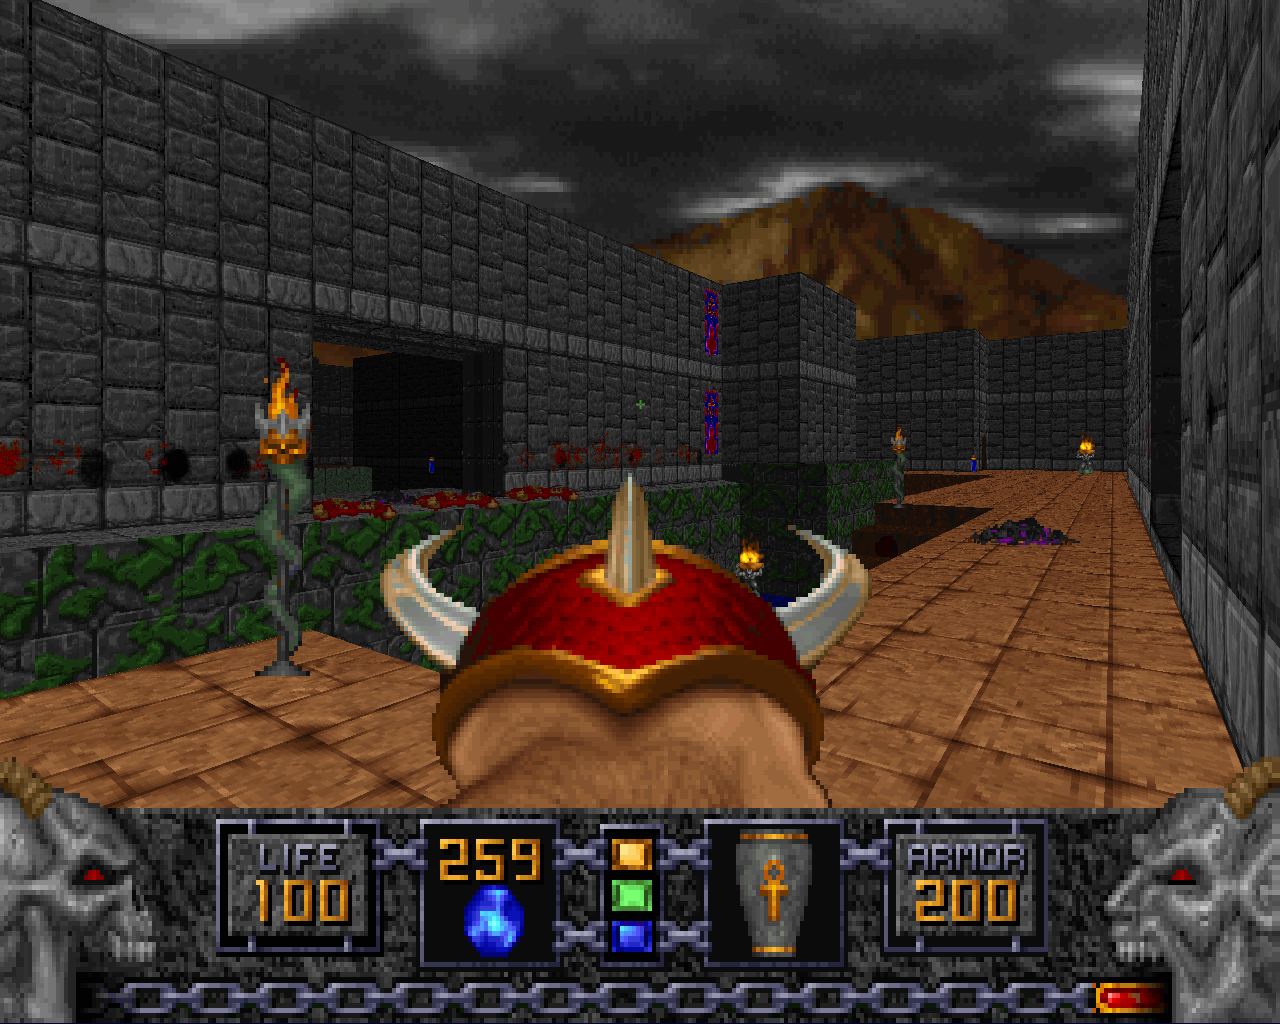
\includegraphics[width=0.8\textwidth]{images/estadodelarte/motores/heretic}
    \caption{\citegame{heretic}, es un juego desarrollado con el motor de Doom.}
\end{figure}

Este concepto inició las comunidades de ``Modding'', que son grupos de aficionados que desarrollaban juegos nuevos modificando juegos antiguos, y para finales de los noventa, juegos como \cite{Quake_3} y \cite{unreal} habían sido diseñados pensando en la reusabilidad de su código. Actualmente, la mayor parte de las compañías desarrolladoras de juegos adquieren la licencia de motores desarrollados por terceros, mucho más económico que desarrollar desde cero todos los componentes.

La linea que separa el motor del juego suele ser difusa y depende en gran medida del juego concreto. El principal factor que se utiliza para distinguir un motor de juego de un juego que haya sido desarrollado de forma ``íntegra'' es la presencia de una Arquitectura orientada a datos. Se trata de un paradigma de programación que se basa en diseñar software con la intención de procesar datos, en lugar de en ejecutar secuencias instrucciones fijas.

Idealmente, debería ser capaz de ``reproducir'' cualquier juego a partir de los datos de su contenido, de la misma forma que un programa reproductor de música leer y reproducir canciones. Sin embargo, en la realidad los motores de juegos suelen estar optimizados para un determinado género juego o una plataforma especifica debido a que de esa forma es posible obtener software más eficiente y con mayores prestaciones, aplicando técnicas y patrones de diseño específicos de esos géneros/plataformas.

\subsubsection{Componentes de un Motor}
Los motores de juego son softwares muy complejos, por lo que suelen estar construidos a partir de módulos independientes, lo que facilita enormemente su mantenimiento. Normalmente, un motor de juegos se compone de los siguientes módulos\cite{game_engine_architecture}:
\begin{itemize}
\item\textbf{El Nucleo}: Se trata de una aplicación compleja que recoge gran cantidad de herramientas y utilidades necesarias para el desarrollo del juego. El núcleo suele incluir una librería de funciones matemáticas, herramientas para la gestión eficiente de memoria, estructuras de datos y clases personalizadas, etc.
\item\textbf{Motor de Renderizado}: Posiblemente el componente más grande y complejo del juego, el motor de renderizado es el software encargado de generar los gráficos del juego. Estos motores suelen estar construidos siguiendo una estructura de capas: primero el \textbf{render de bajo nivel}, que se encarga de dibujar primitivas a la mayor velocidad posible; el \textbf{grafo de escena} determina que sección de la escena es visible, lo que permite reducir el número de llamadas al render de bajo nivel; la capa de \textbf{efectos visuales}, que contiene el sistema de partículas, los efectos de pantalla completa, o las luces dinámicas; y finalmente la capa de \textbf{frontend}, la cual sirve para el renderizado de imágenes 2D que se superpondrán a la escena tridimensional del juego, como los menús, el HUD (Head Up Display) o videos pre-renderizados. Aparte del motor gráfico, los motores de juego actuales suelen incluir también un \textbf{Sistema de Animación}, el cual permita dotar de movimientos naturales a los personajes y elementos del juego. 
\item\textbf{Gestor de Recursos}: Se trata de una interfaz que permite un acceso unificado a los distintos assets que forman el juego (modelos, texturas, sonidos, scripts...). 
\item\textbf{Motor de Físicas}: El motor de físicas permite realizar la detección de colisiones entre entidades del juego, así como la simulación de comportamientos físicos realistas para dichas entidades. Hoy en día, las compañías no suelen programar sus propios motores de físicas, en su lugar adquieren motores desarrollados por terceros, como \textit{Havok}\footnote{https://www.havok.com/physics/} o \textit{PhysX}\footnote{https://www.geforce.com/hardware/technology/physx\#source=gss}.
\item\textbf{Entrada y Salida del Jugador}: Este sistema se encarga de gestionar la información de entrada del jugador, suministrada mediante el mando de juego o el teclado y ratón. El sistema toma la información en bruto de entrada y permite al programador acceder a ella de forma más útil, limpiando los datos de entrada, creando eventos de activación de teclas y proveyendo de sistemas para mapear funciones a distintas teclas o botones y para detectar secuencias de pulsaciones. Este sistema también provee funciones para la salida de datos relacionado con los mandos de control, como activar y desactivar la vibración o emitir sonidos.
\item\textbf{Sistema de Audio}: Es el componente encargado de la reproducción de la música y efectos de sonido del juego. Aunque su complejidad depende en gran medida de las necesidades del motor concreto, la mayoría incluyen sistemas para producir efectos como sonido 3D o música dinámica.
\item\textbf{Networking}: Son los sistemas encargado de realizar la conexión del juego con Internet para, en la mayoría de los casos, realizar partidas en línea con otros jugadores. El soporte de sistemas para el jugo multijugador tiene un gran impacto en la mayoría de componentes del motor, por lo que estos suelen ser desarrollados pensando desde el principio en el modo multijugador, e implementando el modo de un jugador como un caso específico del multijugador.
\item\textbf{Fundamentos de la Jugabilidad}: Esta capa implementa una serie de sistemas que permiten implementar la Jugabilidad. Suele incluir un lenguaje de Scripting, un sistema de eventos, inteligencia artificial, cámaras...
\item\textbf{Herramientas de depuración}: Estas herramientas facilitan la tarea de depurar y optimizar el juego. Incluyen herramientas para dibujar en pantalla, consolas de comandos, sistemas para grabar y reproducir sesiones de juego...
\end{itemize}

\subsection{Ejemplos de Motores}
\subsubsection{Unity 3D}
\textbf{Unity}\footnote{https://unity3d.com/unity}, conocido popularmente como \textbf{Unity3D}, es un motor de juego con su propio Entorno de Desarrollo Integrado (IDE) lanzado en el año 2005 por la compañía Unity Technologies. El desarrollo de este motor comenzó en el año 2002, encabezado por los desarrolladores David Helgason, Joachim Ante y Nicholas Francis. Se trata de uno de los motores más utilizados del mercado, especialmente para el desarrollo de juegos para dispositivos móviles (más del 30\% de los 1000 juegos más exitosos para dispositivos móviles fueros desarrollados con este motor). 
\begin{figure}[h]
	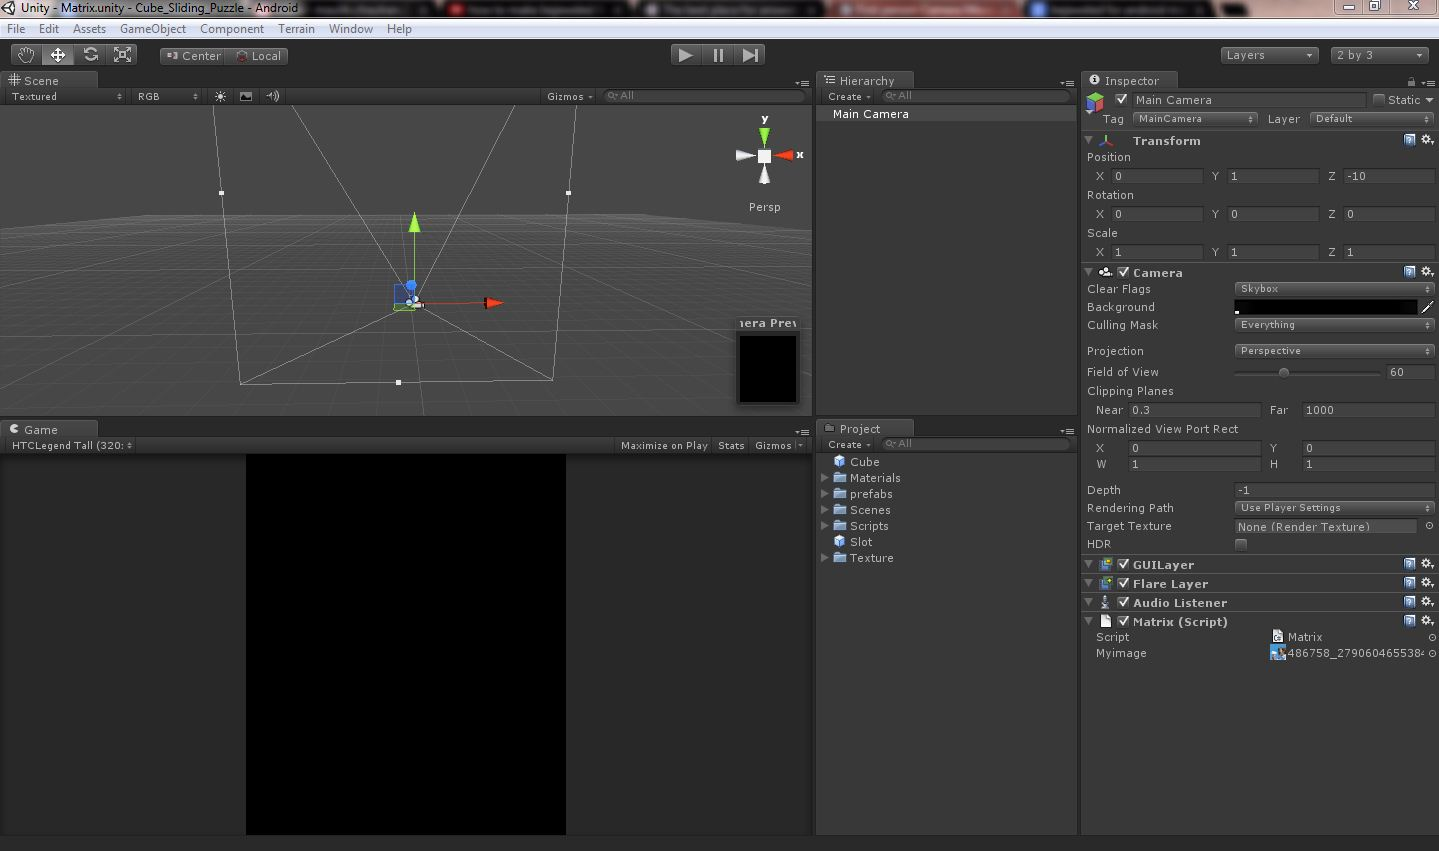
\includegraphics[width=0.8\textwidth]{images/estadodelarte/motores/captura-unity}
	\centering
	\caption{Captura del entorno de desarrollo de Unity}
\end{figure}

La cualidad más importante de Unity es la facilidad de su uso: El motor cuenta con una arquitectura de componentes fácil de entender, el proceso de exportación es muy simple y además cuenta con una tienda de Assets integrada. El Scripting en Unity se realiza en los lenguajes \textbf{C\#} o \textbf{UnityScript} (una variante de JavaScript). Unity ofrece la posibilidad de exportar juegos a 27 plataformas distintas, desde dispositivos móviles a consolas de sobremesa, pasando por los sistemas operativos más comunes de los ordenadores personales. Debido a que su uso es muy extendido, Unity cuenta con una amplia base usuarios, por lo que es sencillo encontrar ayuda en los foros de desarrollo. La facilidad de uso viene a costa de la potencia: su motor gráfico no es tan potente como el de otros motores de la competencia y su rendimiento no es muy óptimo para el desarrollo de juegos de gran envergadura.

\begin{figure}[!htb]
   \begin{minipage}{0.50\textwidth}
     \centering
     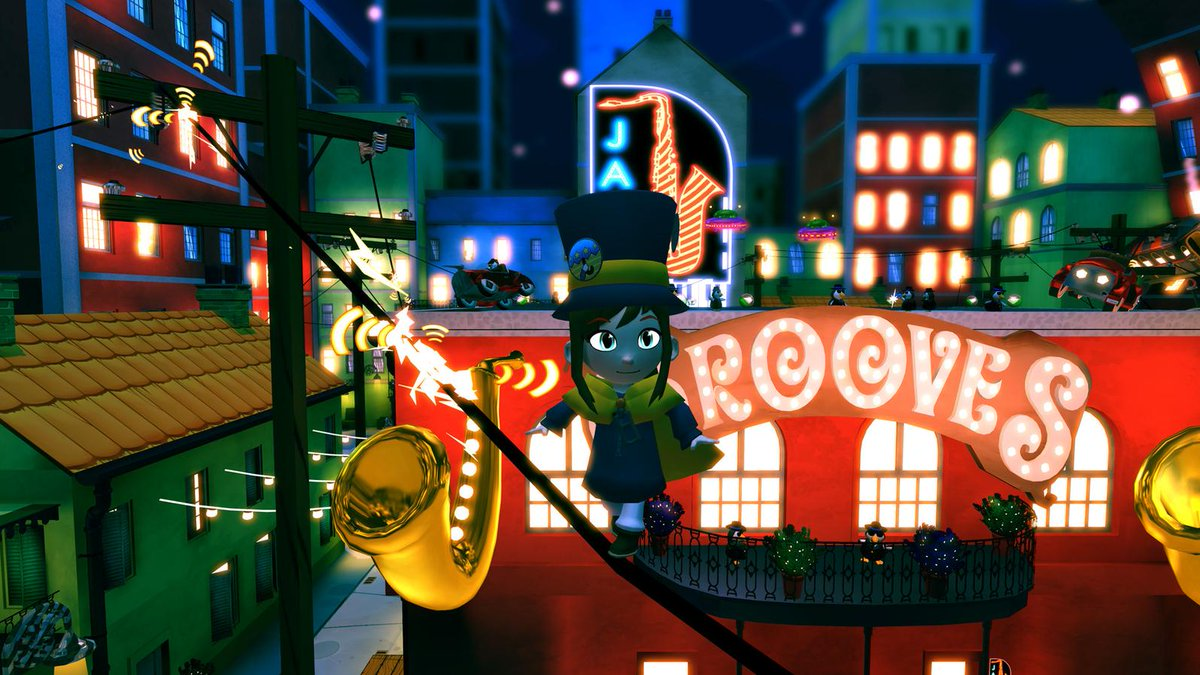
\includegraphics[width=0.9\linewidth, left]{images/estadodelarte/motores/hat-in-time}
     \caption{A Hat in Time (Gears for Breakfast, 2017)}
   \end{minipage}\hfill
   \begin {minipage}{0.50\textwidth}
     \centering
     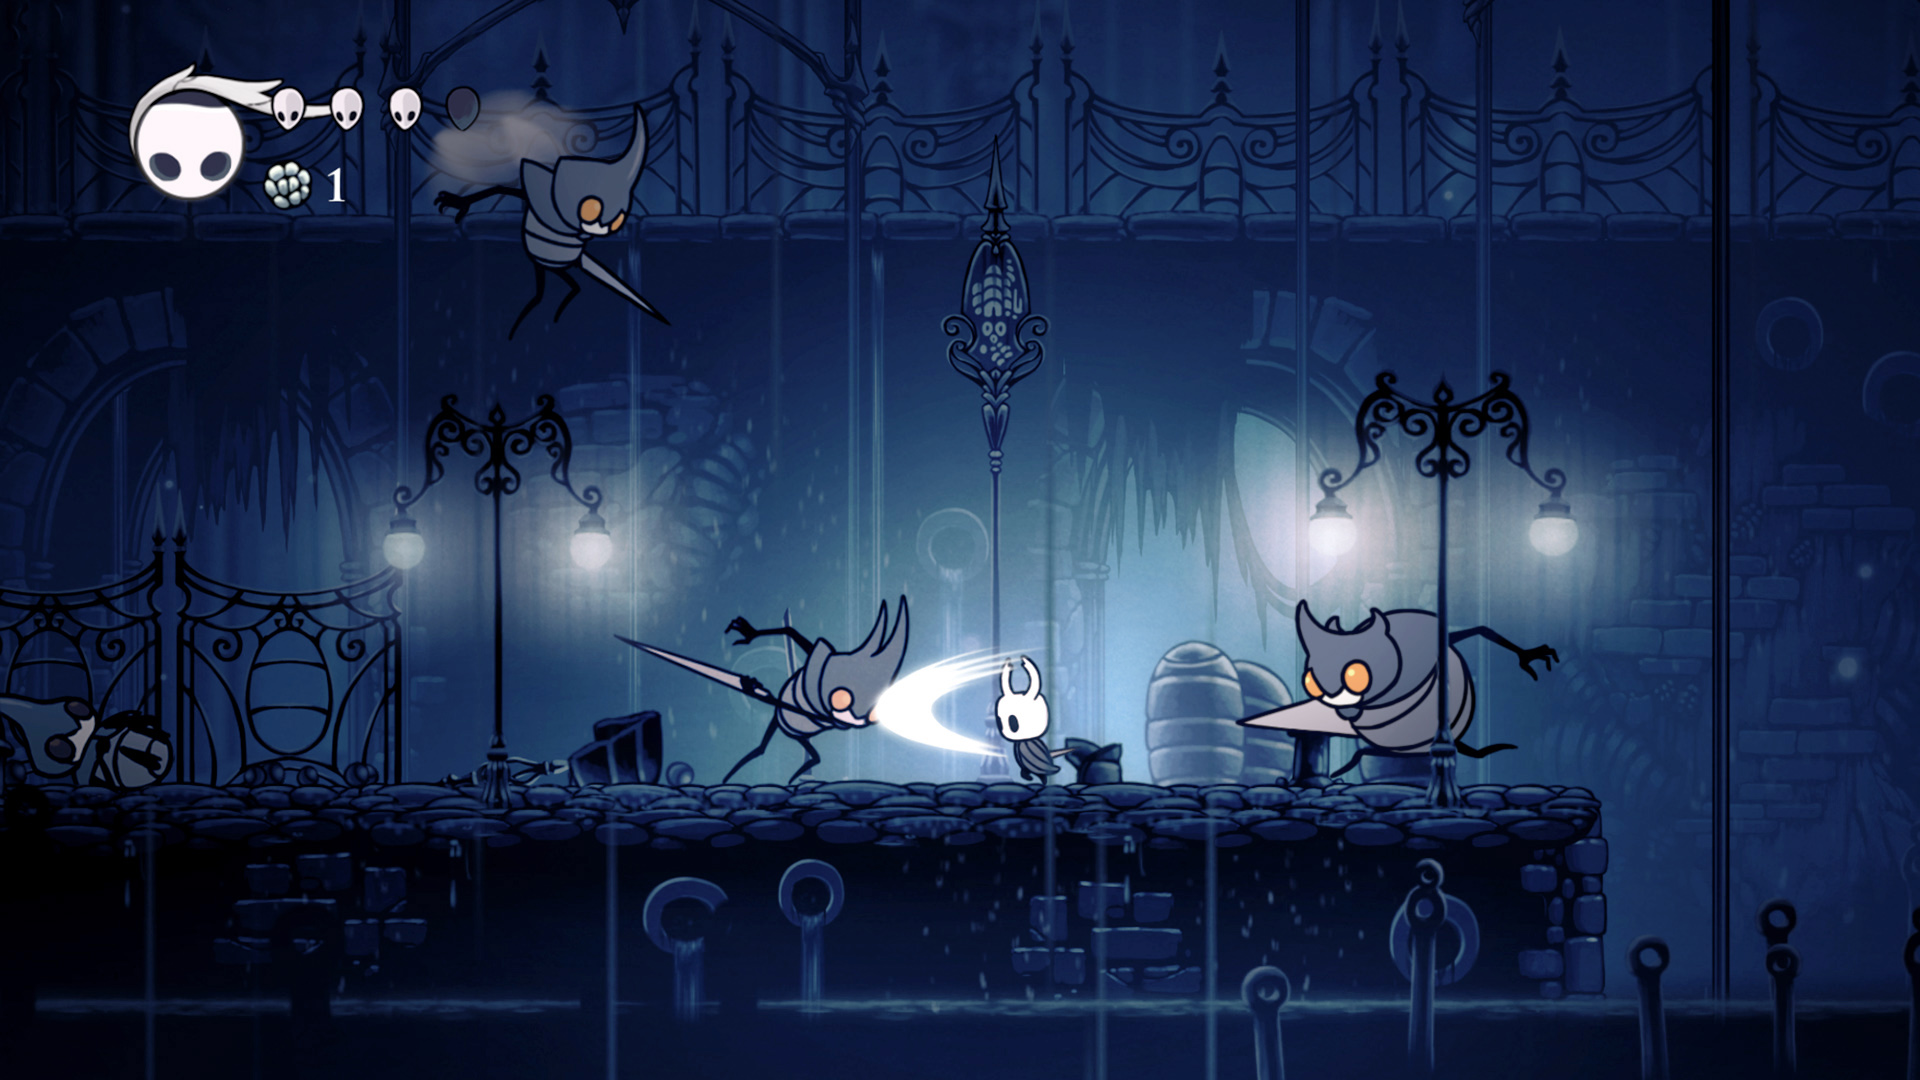
\includegraphics[width=0.9\linewidth, right]{images/estadodelarte/motores/hollow-knight}
     \caption{Hollow Knight (Team Cherry, 2017)}
   \end{minipage}
   \caption{Juegos desarrollados con Unity3D}
\end{figure}

Unity Technologies ofrece distintos planes de pago a los desarrolladores interesados en adquirir la licencia de su motor: La versión gratuita, Unity Personal, que ofrece la funcionalidad básica; Unity Plus que por 35€ al mes ofrece mayor personalización y herramientas de monetización y análisis de rendimiento; y la versión profesional, Unity Pro (125€ al mes) la cual ofrece las prestaciones de la versión Plus más acceso al código fuente y mejor atención al cliente. 

\subsubsection{Unreal Engine}
El \textbf{Unreal Engine}\footnote{https://www.unrealengine.com/} es un popular motor de juego desarrollado por la compañía Epic Games. Originalmente desarrollado como motor propietario para el juego \citegame{unreal}, Epic Games pronto empezó a cerrar tratos con otras compañías que querían utilizar el motor en sus proyectos. Actualmente el motor se encuentra en su versión 4 y es uno de los más populares del sector, habiendo ganado incluso el premio Guinness al "motor de juegos más exitoso" con un total 408 juegos (a fecha de julio de 2014) desarrollados con Unreal. 
\begin{figure}[h]
	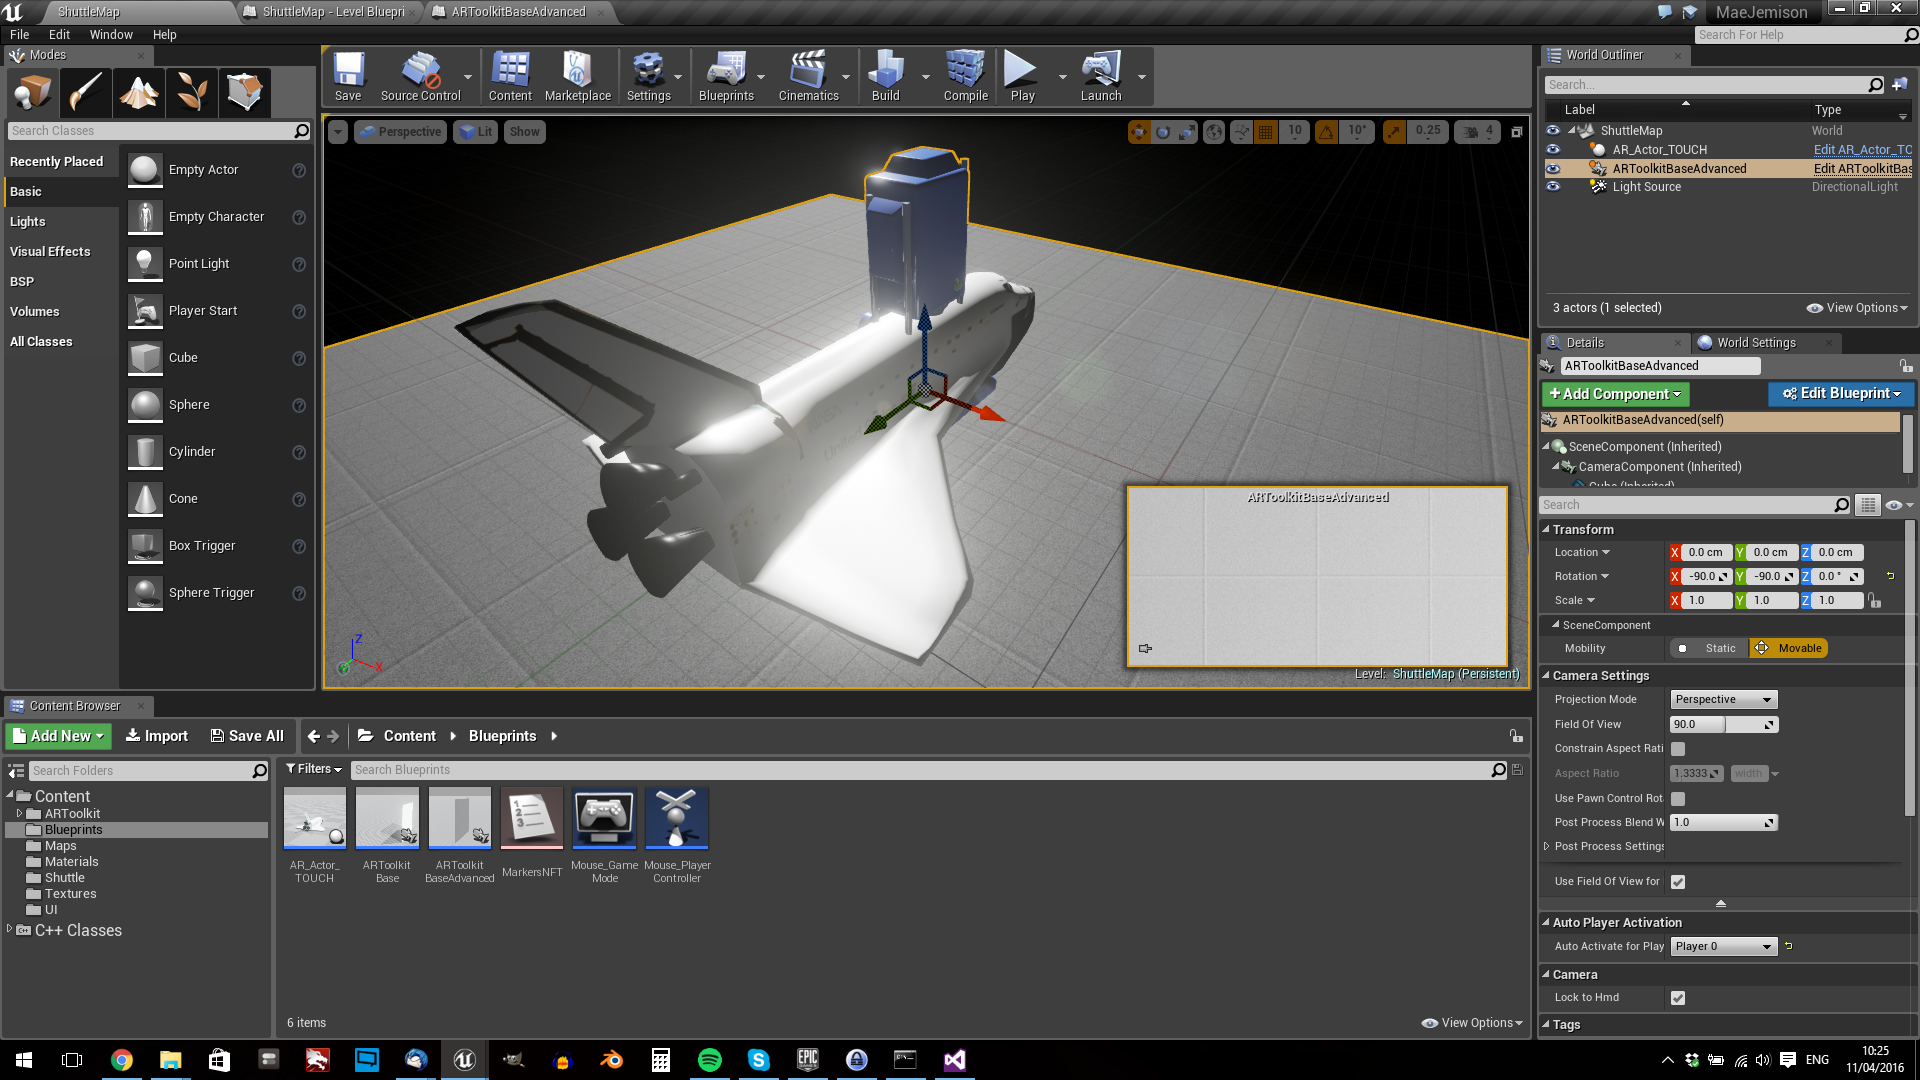
\includegraphics[width=0.8\textwidth]{images/estadodelarte/motores/captura-unreal}
	\centering
	\caption{Captura del entorno de Unreal Engine}
\end{figure}

Unreal Engine es un motor orientado al desarrollo de juegos ``AAA'', proyectos de gran envergadura llevados por equipos grandes. Uno de sus puntos fuertes es su potente motor de rendering el cual da soporte a gráficos fotorrealistas y permite el uso de efectos de post-procesados complejos entre otras características. El scripting en Unreal se realiza mediante el sistema \textbf{Blueprint} de Scripting visual, el cual permite programar conectando de forma gráfica bloques de código. El motor permite también escribir código directamente en C++, lo que aumenta su flexibilidad. El paquete de herramientas del motor también incluye programas como generadores de terreno, editores de materiales, herramientas para animación... Sin embargo, se trata de un motor complicado y difícil de aprender a utilizar, además de que la potencia que requiere lo hace poco adecuado para el desarrollo para plataformas móviles.

\begin{figure}[!htb]
   \begin{minipage}{0.5\textwidth}
     \centering
     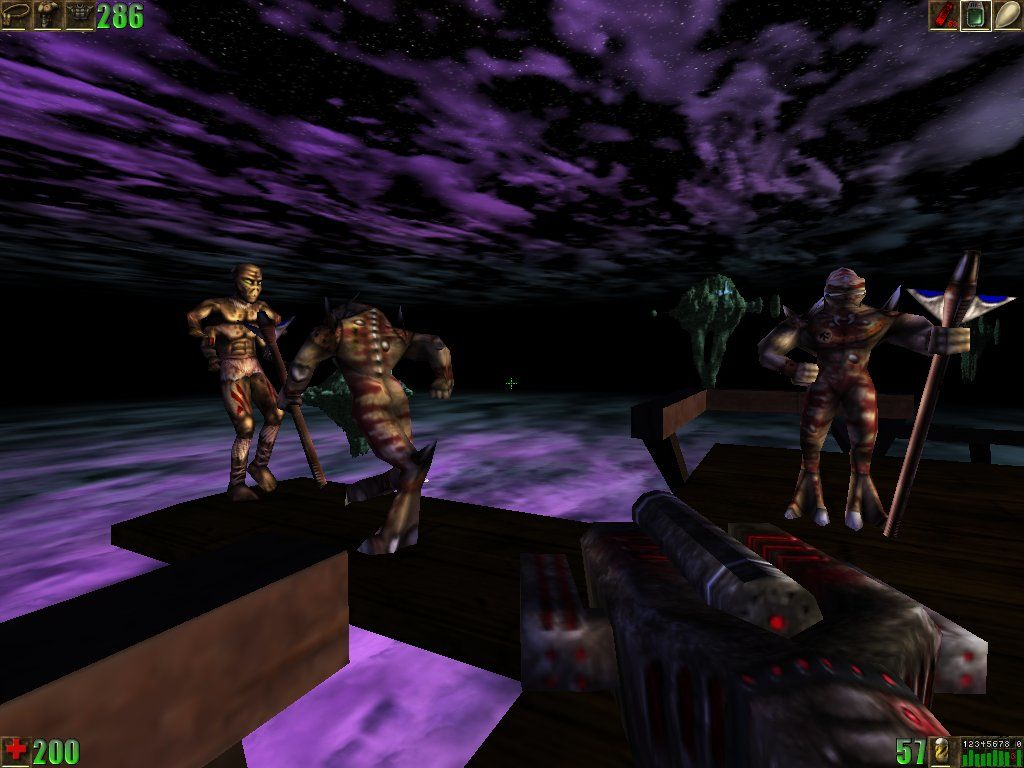
\includegraphics[width=0.85\linewidth, right]{images/estadodelarte/motores/unreal-original}
     \caption{Unreal (Epic Games, 1998)}
   \end{minipage}\hfill
   \begin {minipage}{0.5\textwidth}
     \centering
     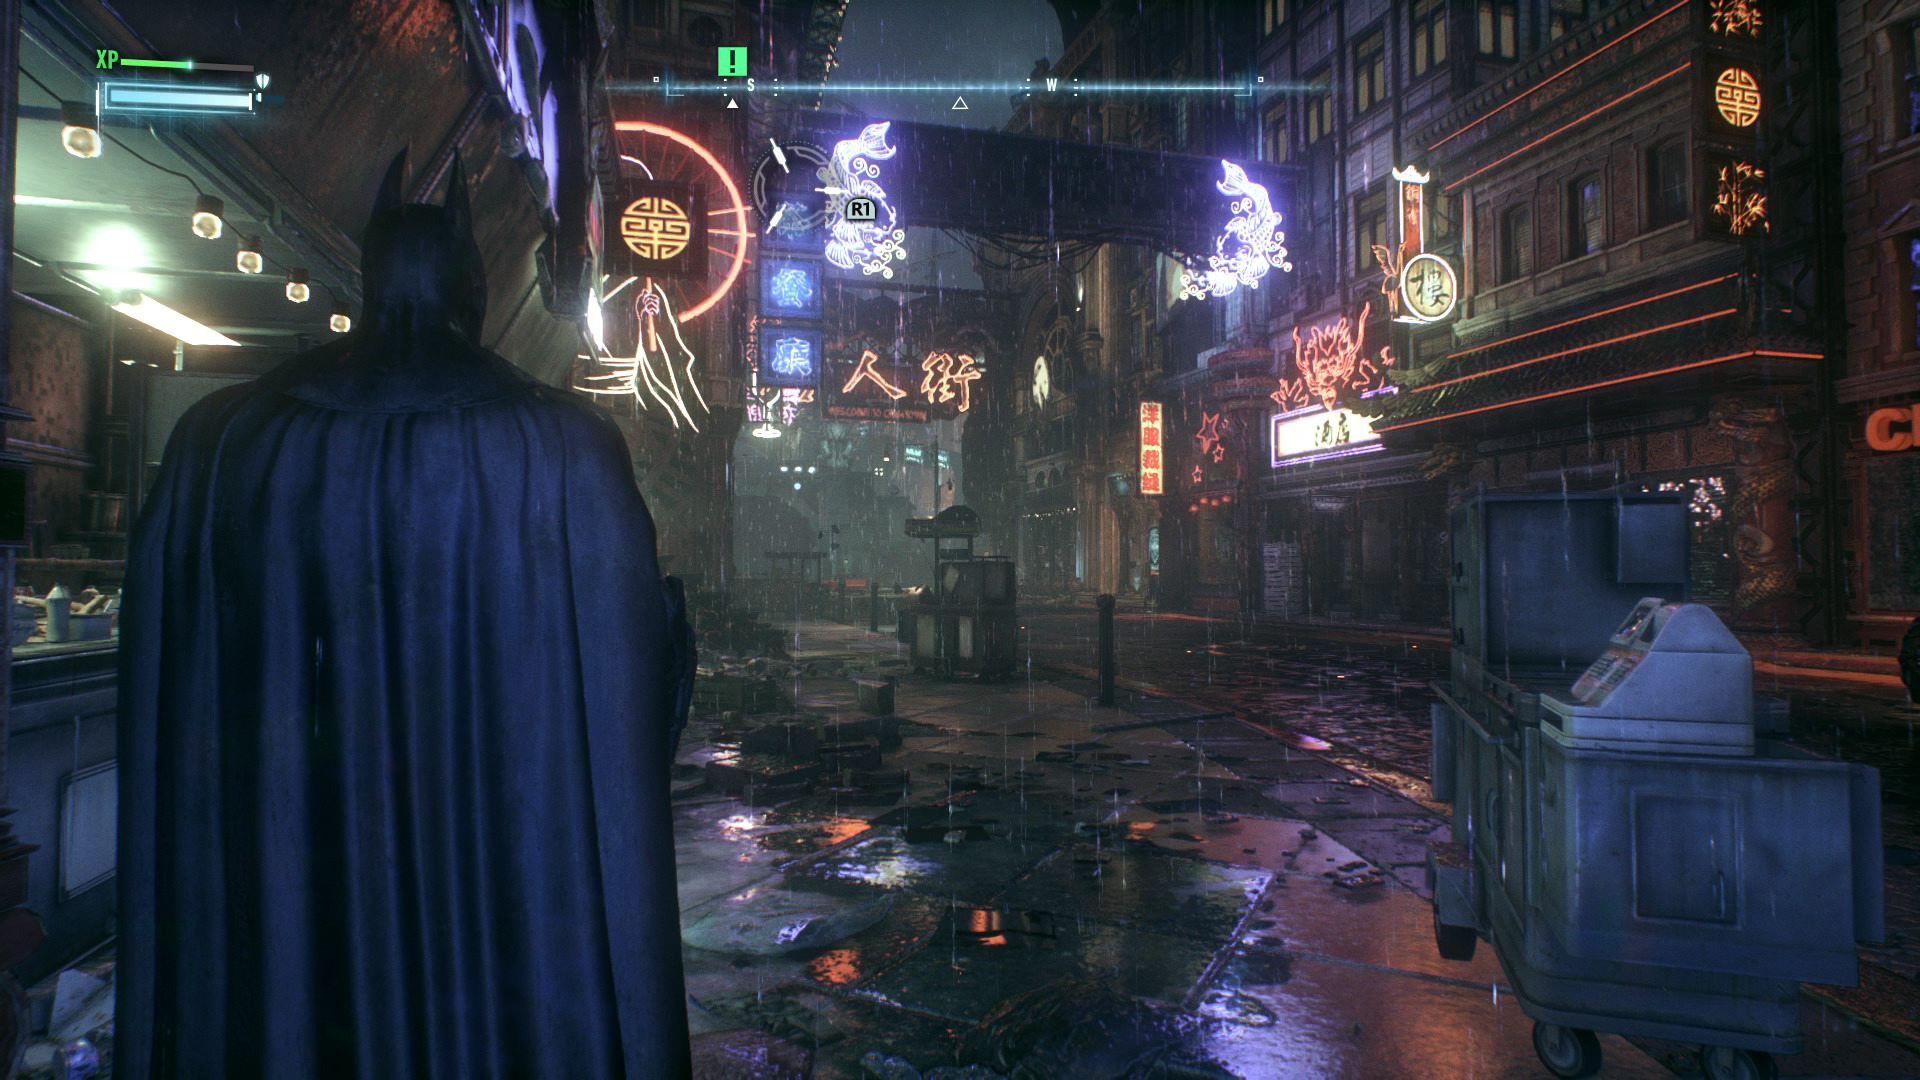
\includegraphics[width=0.85\linewidth, left]{images/estadodelarte/motores/batman-arkham}
     \caption{Batman: Arkham Knight (Rocksteady Studios, 2015)}
   \end{minipage}
   \caption{Juegos desarrollados con Unreal Engine}
\end{figure}

La licencia de uso de Unreal Engine es gratuita, sin embargo, en proyectos comerciales Epic Games cobra un 5\% de las ganancias a partir de los 3.000\$ por trimestre. En casos especiales, es posible negociar otros tipos de licencias con Epic Games.

\subsubsection{Game Maker Studio}
\textbf{Game Maker Studio}\footnote{https://www.yoyogames.com/gamemaker} es un motor de juegos desarrollado por Yoyo Games. El programa fue lanzado originalmente en 1994 bajo el nombre de \textbf{Amino} como una herramienta para la creación de animaciones. Desde entonces, el programa ha ido evolucionado hasta convertirse en un motor de juegos de calidad profesional.
\begin{figure}[h]
	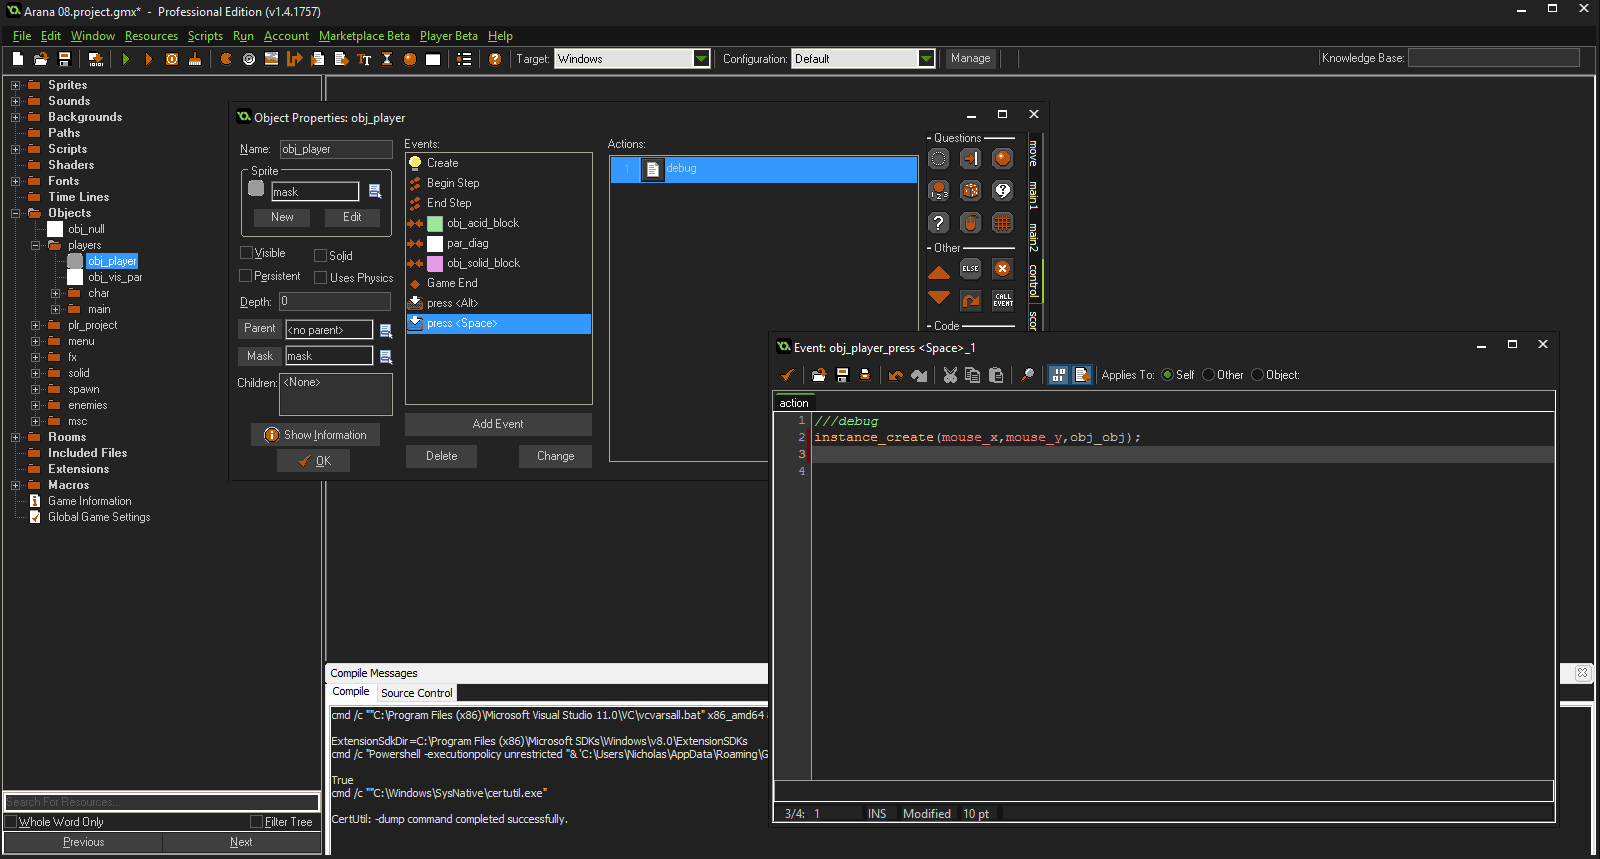
\includegraphics[width=0.8\textwidth]{images/estadodelarte/motores/captura-game-maker}
	\centering
	\caption{Captura del entorno de Game Maker Studio}
\end{figure}

Game Maker Studio está diseñado para ser muy sencillo de usar: su principal uso es como una herramienta para gente sin conocimientos de programación, la cual permite desarrollar juegos sin necesidad de escribir una línea de código; o para el desarrollo rápido de juegos pequeños o prototipos. La programación de scripts en Game Maker se realiza mediante el sistema \textbf{``Drag and Drop''}, con el que se programa conectando diversos bloques de código; o el mediante un lenguaje de programación propio llamado \textbf{Game Maker Language}. El motor permite exportar con facilidad a distintas plataformas como PC, dispositivos móviles o HTML5. El entorno integrado de Game Maker incluye herramientas complementarias como un editor gráfico y un editor de mapas para centralizar el desarrollo. Sin embargo, la sencillez del motor también se refleja en su potencia: Game Maker Studio carece de soporte para gráficos tridimensionales complejos, y su arquitectura dificulta el desarrollo de proyectos de gran envergadura.

\begin{figure}[!htb]
   \begin{minipage}{0.5\textwidth}
     \centering
     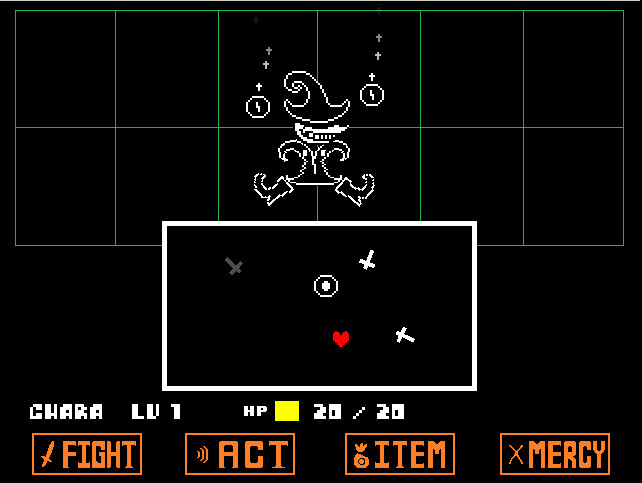
\includegraphics[width=0.85\linewidth, right]{images/estadodelarte/motores/undertale}
     \caption{Undertale (Toby Fox, 2015)}
   \end{minipage}\hfill
   \begin {minipage}{0.5\textwidth}
     \centering
     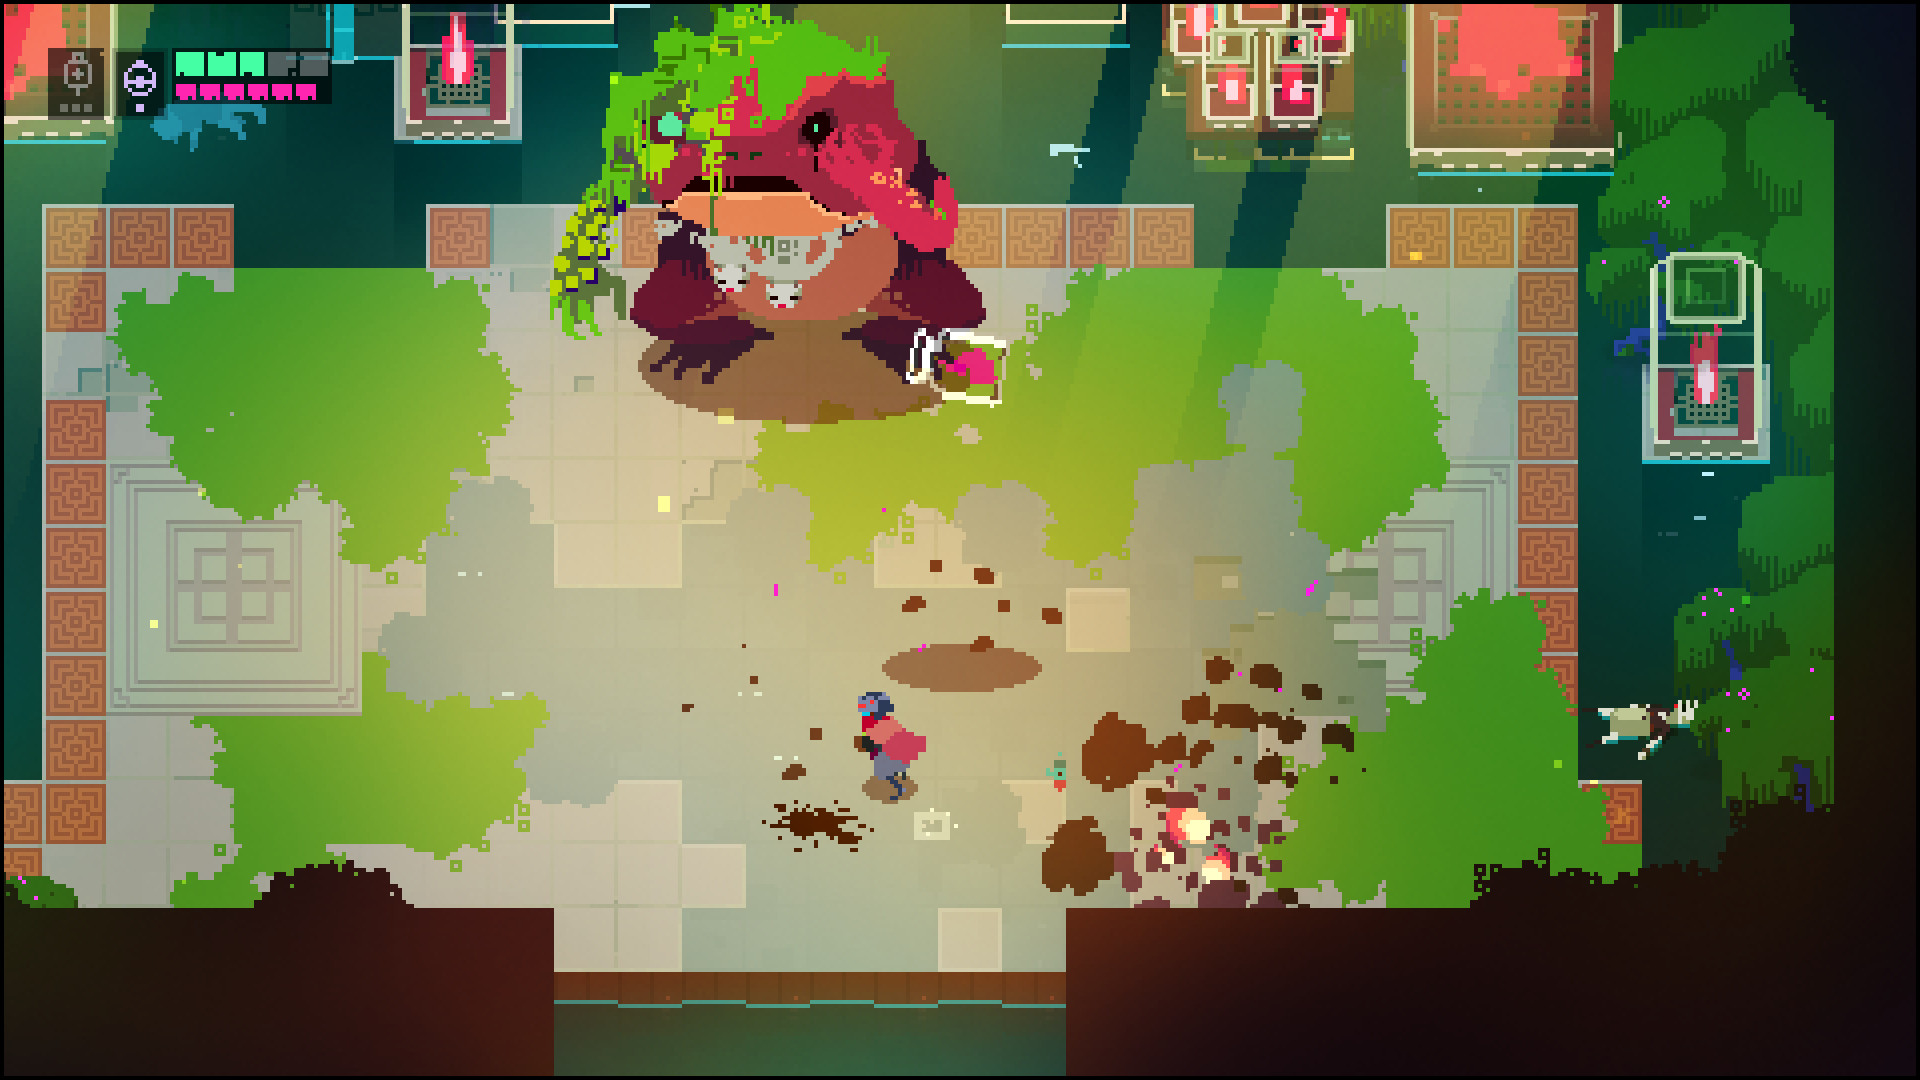
\includegraphics[width=0.85\linewidth, left]{images/estadodelarte/motores/hyper-light-drifter}
     \caption{Hyper Light Drifter (Heart Machine, 2016)}
   \end{minipage}
   \caption{Juegos desarrollados con Game Maker}
\end{figure}

La licencia de la versión actual de Game Maker Studio (Game Maker Studio 2) se encuentra a la venta por distintos precios dependiendo de la plataforma de distribución para la que se quiera trabajar: desde la versión básica por 39\$ anuales hasta la versión profesional permanente con posibilidad de exportación a IOS, Android y consolas por 399\$. Existen también una versión de prueba gratuita que cuenta con unas prestaciones reducidas y un plan de pago para su uso en centros educativos.
